In order to have a sound and accurate upper bound on the  adaptivity of a program $c$,
we design a program analysis framework named {\THESYSTEM}.
This framework composes two algorithms as shown in the double-stroke box and the dashed box in Fig.~\ref{fig:adaptfun}.
The first algorithm in the double-stroke box combines the quantitative and dependency analysis techniques.
It produces an estimated \emph{data-dependency graph} for a program.
The second algorithm in the dashed box is a walk length estimation algorithm.
%  in the dashed box in Fig.~\ref{fig:adaptfun}.
It computes the upper bound on the program's \emph{adaptivity} over the estimated graph.
%  of the adaptive data analysis program $c$.
\begin{figure}
  \centering    
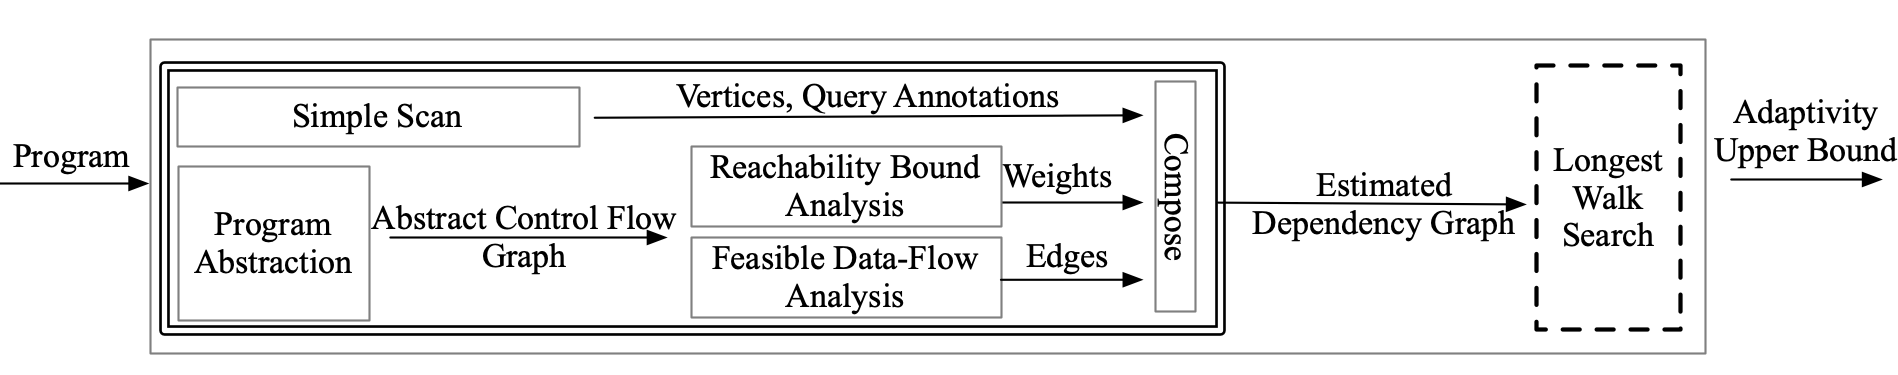
\includegraphics[width=1.0\columnwidth]{adaptfun.png}
  \vspace{-0.3cm}
  \caption{The overview of {\THESYSTEM}}
  \label{fig:adaptfun}
  \vspace{-0.5cm}
\end{figure}
%
Below is the outline of the {\THESYSTEM}.
% through Section~\ref{sec:alg_vertexgen}, Section~\ref{sec:alg_weightedgegen} and~\ref{sec:alg_graphgen}:
\begin{enumerate}
  \item \textbf{Graph Estimation}
  Because adaptivity is defined over a program's \emph{quantitative dependency graph} (in Definition~\ref{def:trace_graph}),
  this algorithm first estimates this graph for the program statically
  in Section~\ref{sec:alg_graphgen}.
  It estimates the four components of this graph in two steps and then composes them into an estimated dependency graph
  %  for a program 
  in the last step.
  The steps are summarized  as follows.
\begin{enumerate}
  \item \textbf{Vertex and Query Annotation Estimation}
  Vertices and query annotations in this graph are the assigned variables with unique labels. These are extracted directly from the program as in Section~\ref{sec:alg_vertexgen}.
  \item \textbf{Edge and Weight Estimation}
  \\
  This step estimates the edge and weight for a quantitative dependency graph. It combines the control, data-flow  analysis algorithm and the loop bound inference algorithm.
  There are three computation steps in this algorithm.
  \\
  \textbf{Abstract Control Flow Graph.}
  In order to perform the dependency analysis and quantitative analysis, this step first generates an \emph{abstract control flow graph} for a program in Section~\ref{sec:alg_abscfg}.
  \\
  \textbf{Edges Estimation via Combined Flow Analysis.} 
  The step is presented in
  Section~\ref{sec:alg_edgegen}. It performs over the \emph{abstract control flow graph}, which combines both control flow and data flow analysis.
  It estimates the \emph{dependency relation} between each pair of the labeled variables in a program by considering both the control flow and data flow.
  Then it uses the estimated dependency relation to approximate the edge
  %  of the quantitative dependency graph 
  between each pair of vertices.
  \\
  \textbf{Weights Estimation via Quantitative Analysis.} 
  This step is presented in Section~\ref{sec:alg_weightgen}. 
  It performs over the same \emph{abstract control flow graph} and computes the upper bound on the maximal visiting times of each labeled variable for a program.
  It estimates the reachability bound for every vertex over the \emph{abstract control flow graph},
  and this reachability bound is used to estimate the maximal visiting times of each labeled variable in a program and the weight of the corresponding vertex.
  %  of this quantitative dependency graph.
\item  \textbf{Graph Estimation.} 
In Section~\ref{sec:alg_graphgen}, we construct the final approximated graph,
named \emph{estimated dependency graph} by simply composing the four estimated ingredients. 
Overall, this \emph{estimated dependency graph} has a similar topology structure as 
the \emph{semantics-based dependency graph}. It has the same
vertices and query annotations, but approximated edges and weights. 
\end{enumerate}

\item \textbf{Adaptivity Computation.} 
Likewise the adaptivity in Definition~\ref{def:trace_adapt},
%  is defined as a finite walk in the \emph{semantics based dependency graph}, 
the static estimation on the \emph{adaptivity} also relies on finding a walk in the \emph{estimated dependency graph}.  
We discuss some challenges in finding the 'appropriate' walk in the graph, and how our algorithm responds to these challenges as
% . We present the path searching algorithm 
in Section~\ref{sec:alg_adaptcompute}.
\end{enumerate}